\documentclass[10pt,a4paper]{article}

\usepackage[utf8]{inputenc}
\usepackage{cmap}
\usepackage[T1]{fontenc}
\usepackage[scaled=0.95]{helvet}
\renewcommand{\familydefault}{\sfdefault}
\usepackage[spanish]{babel}
\usepackage[a4paper,margin=1.55cm]{geometry}
\usepackage{graphicx}
\usepackage{xcolor}
\usepackage{enumitem}
\usepackage{needspace}
\usepackage[colorlinks=true,urlcolor=accent,linkcolor=accent,citecolor=accent]{hyperref}

\definecolor{navy}{HTML}{16344A}
\definecolor{accent}{HTML}{16877A}
\definecolor{pale}{HTML}{EDF4F3}
\definecolor{muted}{HTML}{5C6B73}

\setlength{\parindent}{0pt}
\setlength{\parskip}{1pt}
\setlist[itemize]{label={\large\textbullet},leftmargin=1.35em,itemsep=1pt,topsep=2pt}
\urlstyle{same}

\newcommand{\cvsection}[1]{%
    \vspace{11pt}%
    {\large\bfseries\color{navy}#1}\par
    \vspace{2pt}{\color{accent}\rule{\linewidth}{1.2pt}}\par
    \vspace{5pt}%
}

\begin{document}

\noindent
\colorbox{navy}{%
    \begin{minipage}{\dimexpr\textwidth-2\fboxsep\relax}
        \color{white}
        \begin{minipage}[c]{0.72\linewidth}
            {\fontsize{18}{21}\selectfont\bfseries CARLOS ALEJANDRO FREITAS TEIXEIRA}\par
            \vspace{3pt}
            {\large\bfseries\color{pale}Ingeniero de Sistemas | Máster en Inteligencia Artificial}\par
            \vspace{7pt}
            {\small Porto, Portugal \textbar{} \href{mailto:carlosfreitasingsistemas@gmail.com}{\textcolor{white}{carlosfreitasingsistemas@gmail.com}} \textbar{} +351 937797609\par}
            \vspace{3pt}
            {\small
                \href{https://github.com/CarlosFreitasING}{\textcolor{white}{GitHub}}
                \textcolor{pale}{\textbar{}}
                \href{https://www.linkedin.com/in/carlos-alejandro-freitas-teixeira-82921a249/}{\textcolor{white}{LinkedIn}}
                \textcolor{pale}{\textbar{}}
                \href{https://carlosfreitas32.wixsite.com/portafolio}{\textcolor{white}{Portafolio}}
            }
        \end{minipage}
        \hfill
        \begin{minipage}[c]{0.22\linewidth}
            \centering
            \fcolorbox{white}{pale}{%
                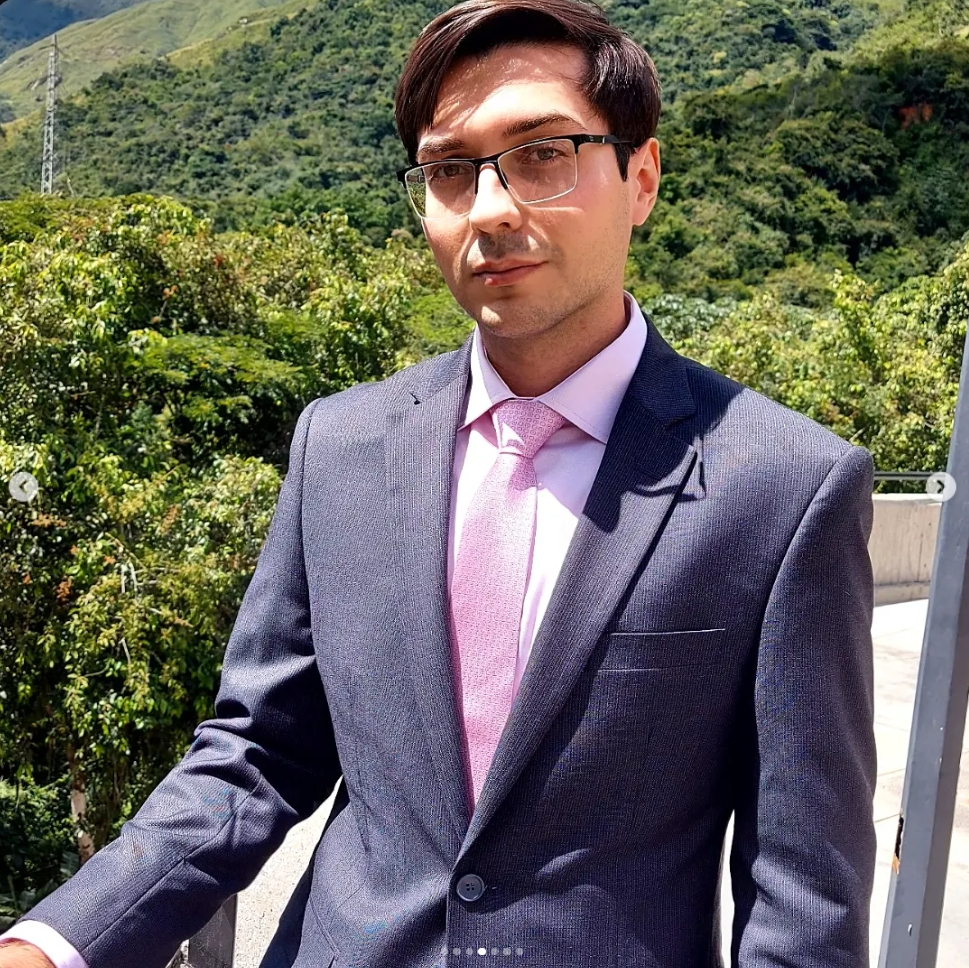
\includegraphics[width=3.2cm,height=3.2cm,keepaspectratio,trim=6cm 12cm 6cm 0cm,clip]{assets/foto.jpeg}%
            }
        \end{minipage}
    \end{minipage}%
}

\cvsection{PERFIL}
\colorbox{pale}{%
    \parbox{\dimexpr\textwidth-2\fboxsep\relax}{%
        Ingeniero de Sistemas y Máster en Inteligencia Artificial con experiencia en investigación aplicada (I+D) de soluciones basadas en IA. Poseo sólidos conocimientos en Computer Vision, Machine/Deep Learning, LLMs, Edge AI y Robótica (ROS 2), complementados con experiencia práctica en desarrollo full-stack. Orientado a diseñar arquitecturas escalables, implementar modelos de inferencia local y desplegar soluciones tecnológicas en entornos reales orientados al usuario.
    }%
}

\cvsection{EXPERIENCIA}

\Needspace{4\baselineskip}
\textbf{\large Investigador y Desarrollador de Inteligencia Artificial (I+D)}\\
{\color{muted}GECAD - ISEP \textbar{} Porto, Portugal}

\vspace{4pt}
\textbf{\color{accent}Proyecto CRIARTE \textbar{} Oct 2025 -- Presente}\\
Contribuyo a un proyecto europeo de innovación que busca transformar la industria de la construcción mediante IA, robótica y tecnologías emergentes, en el marco de la Industria 5.0.
\begin{itemize}
    \item Investigo, entreno y evalúo modelos de Machine Learning y algoritmos de clustering para analizar datos de sensores vestibles e identificar patrones asociados a los estados fisiológicos de los trabajadores.
    \item Ajusto modelos YOLO mediante fine-tuning para detectar personas y estimar la pose humana con sistemas de visión por computadora.
    \item Desarrollo arquitecturas distribuidas basadas en ROS 2 para integrar sistemas de visión artificial y monitorización fisiológica.
    \item \textbf{Stack Tecnológico:} ROS 2, YOLO, ReID, Computer Vision, Machine Learning, GMM, AHC, Python, C++.
\end{itemize}

\vspace{2pt}
\textbf{\color{accent}Proyecto WAI (Wellbeing@Artificial Intelligence) \textbar{} Nov 2025 -- Jun 2026}\\
Participé en una iniciativa europea de investigación que utiliza soluciones de Inteligencia Artificial para fomentar el bienestar estudiantil y apoyar la gestión de la ansiedad y la salud mental.
\begin{itemize}
    \item Desarrollé y publiqué la aplicación móvil ``WellBe'' para \href{https://play.google.com/store/apps/details?id=com.caloale.waiv1\&hl=en_US}{Android} e \href{https://apps.apple.com/ie/app/wellbe-journaling-app/id6758772082}{iOS}.
    \item Alcancé un despliegue internacional, con usuarios en 7 países y más de 200 descargas.
    \item Implementé modelos de IA con inferencia local mediante una arquitectura offline-first para proteger la privacidad de los usuarios.
    \item \textbf{Stack Tecnológico:} React Native, Expo, EAS Build, SQLite, ONNX Runtime, TinyBERT.
\end{itemize}

\Needspace{4\baselineskip}
\textbf{\large Desarrollador de Software Freelance}\\
{\color{muted}Remoto \textbar{} Oct 2022 -- Presente}
\begin{itemize}
    \item Diseño y desarrollo soluciones full-stack para clientes y empresas, digitalizando y automatizando procesos.
    \item Desarrollé plataformas web y sistemas de gestión, incluida una aplicación de fidelización digital para un negocio de restauración (Ver: \href{https://avenidakebab.com/}{Web de fidelización}).
    \item Diseñé bases de datos, configuré la autenticación de usuarios y la gestión de permisos, e integré servicios mediante APIs.
    \item \textbf{Stack Tecnológico:} Angular, React, PWA, iOS/Android, SQL, RLS, APIs y microservicios.
\end{itemize}

\Needspace{4\baselineskip}
\textbf{\large Programador y Analista Junior Full-Stack}\\
{\color{muted}INFOCENT C.A. \textbar{} Caracas, Venezuela \textbar{} Oct 2023 -- Sep 2024}
\begin{itemize}
    \item Participé en la modernización de una aplicación legacy de gestión de nóminas para clientes empresariales.
    \item Desarrollé e implementé nuevas funcionalidades de frontend y backend para el sistema de nómina.
    \item Realicé mantenimiento correctivo, resolví incidencias y optimicé funcionalidades del sistema.
    \item \textbf{Stack Tecnológico:} Angular, Spring Boot, Java, SQL, Bases de Datos Relacionales.
\end{itemize}

\Needspace{4\baselineskip}
\textbf{\large Desarrollador de Software y Diseñador de Transformación Digital}\\
{\color{muted}Universidad Metropolitana (UNIMET) \textbar{} Caracas, Venezuela \textbar{} 2021 -- 2022}
\begin{itemize}
    \item Lideré la transformación digital y automaticé el sistema de solicitudes académicas, erradicando los cuellos de botella administrativos, optimizando los flujos de trabajo y suprimiendo el procesamiento manual de trámites.
    \item Diseñé y desarrollé una plataforma web interactiva full-stack para la autogestión estudiantil, con notificaciones en tiempo real y un panel de administración.
    \item Desplegué el software en producción y conseguí una adopción sostenida por parte de la comunidad universitaria. La plataforma está en uso desde 2022 (Ver: \href{https://script.google.com/macros/s/AKfycbw3h26r_mjt0jow79RT9dnPaUKZ81dVUsF8qDeEjp7wsRg-ldqHjlB9L0FJYP_Uc_LXUw/exec}{Web Control de Estudio}).
    \item \textbf{Stack Tecnológico:} Google Apps Script, JavaScript, HTML/CSS, Google Sheets, SQL.
\end{itemize}

\cvsection{EDUCACIÓN}
\textbf{Máster en Inteligencia Artificial \textbar{} Instituto Superior de Engenharia do Porto (ISEP)}\\
{\color{muted}Porto, Portugal \textbar{} 2024 -- Oct 2026 (completado)}\\
Tesis defendida: ``Análise e Previsão do Estado Fisiológico de Trabalhadores em Obra através de Gémeos Digitais Humanos e Aprendizagem Automática'' (\href{https://drive.google.com/file/d/1xlqiDRtNX2Xj5_9TnHy6inUlAnseSHbF/view?usp=drive\_link}{PDF de la tesis}).

\vspace{5pt}
\textbf{Ingeniería de Sistemas \textbar{} Universidad Metropolitana (UNIMET)}\\
{\color{muted}Caracas, Venezuela \textbar{} 2016 -- 2022}\\
Tesis de grado: ``Aplicación web para la gestión de solicitud y seguimiento de documentos académicos de la Universidad Metropolitana'' (\href{https://unimet.ent.sirsi.net/client/es_ES/default/search/detailnonmodal/ent:\%24002f\%24002fSD\_ILS\%24002f0\%24002fSD\_ILS:132264/one}{registro en catálogo UNIMET}).

\cvsection{PUBLICACIONES Y CONFERENCIAS}
\begin{itemize}
    \item \textbf{Artículo:} ``A Review of Physiological Monitoring and Prediction in Workers in High-Risk Construction Environments'', presentado en INISTA 2026 (Guimarães, Portugal, 17--19 de septiembre de 2026). Enlaces: \href{https://inista2026.di.uminho.pt/pdf/INISTA\_Official\_Program.pdf}{programa oficial} | \href{https://drive.google.com/file/d/1Kh2M0t4dUh3F5vFrKY5sZMfaRxV1H2PT/view?usp=sharing}{PDF del artículo}.
    \item \textbf{Ponente invitado:} ``Artificial Intelligence in Health and Mental Health: Challenges, Opportunities and Future Perspectives'', en el evento final de difusión del proyecto Erasmus+ WELLBEING@ARTIFICIAL INTELLIGENCE (ISEP, Porto, Portugal, 9--10 de julio de 2026).
\end{itemize}

\cvsection{HABILIDADES TÉCNICAS}
\begin{itemize}
    \item \textbf{Inteligencia Artificial \& Datos:} Computer Vision, Pose Estimation (YOLO), ReID, NLP, LLMs, Fine-tuning, Edge AI, ONNX Runtime, PyTorch, OpenCV, Machine Learning (ANN, CNN, RNN), Clustering (GMM/AHC).
    \item \textbf{Lenguajes de Programación:} Python, TypeScript, JavaScript, Java, C++, C\#, HTML/CSS.
    \item \textbf{Desarrollo y Arquitectura:} React Native, Angular, Spring Boot, ASP.NET, Flutter, Arquitecturas Offline-first / Local-first, Serverless, ROS 2, PWA.
    \item \textbf{Bases de Datos \& Herramientas:} PostgreSQL, Supabase, SQLite, MySQL, MongoDB, SQL Server, Firebase, Git.
\end{itemize}

\cvsection{CERTIFICACIONES}
Certificado de nivel C1 de inglés y certificado de nivel conversacional \textbar{} Fyr Lois \textbar{} 2019 -- 2022.

\vspace{4pt}
Certificados de competencia \textbar{} Universidad Metropolitana \textbar{} 2022
\begin{itemize}
    \item Analista de Sistemas de Información.
    \item Analista en Diseño y Procesamiento de Datos.
    \item Asistente de Ingeniero en Investigación de Operaciones Básico.
    \item Analista de Redes.
\end{itemize}

\cvsection{IDIOMAS}
\textbf{Español:} nativo \hfill
\textbf{Inglés:} C1 \hfill
\textbf{Portugués:} conversacional

\end{document}
